%\documentclass[preprint,review,12pt]{elsarticle}
\documentclass{elsarticle}

\usepackage{graphicx} % Graphics
\usepackage{amssymb} % Various useful mathematical symbols
\usepackage{amsmath} % Advanced quations, including text and align
\usepackage{siunitx} % SI units
\usepackage{lineno} % Line numbers
\usepackage{url} % URL typesetting
\usepackage{tablefootnote} % Footnotes in tables

\journal{Remote Sensing of Environment}

\begin{document}

\begin{frontmatter} % Title, authors and addresses

\title{Investigating the information content of spectral data}
\author[ANS,MCD,SPS]{Alexey N. Shiklomanov, Michael C. Dietze, Shawn P. Serbin}
\address[ANS,MCD]{Dept. of Earth and Environment, Boston University}
\address[SPS]{Brookhaven National Lab}

\begin{abstract}
Abstract...
\end{abstract}

\begin{keyword}
Spectra \sep PROSPECT \sep Leaf
\end{keyword}

\end{frontmatter}

\linenumbers %% Begin line numbering

\section{Introduction} \label{s:intro}
    The biosphere as we know it is fundamentally dependent on the interactions 
    between plants and solar radiation through photosynthesis. Consequently, we 
    can learn a lot about the condition of plants by studying these 
    interactions in detail. Over the last several decades, our capability to do 
    so has expanded dramatically. At regional and global scales, we have used
% * <alexey.shiklomanov@gmail.com> 2018-04-07T17:05:04.796Z:
% 
% > At regional and global scales
% Here is a comment.
% 
% ^ <alexey.shiklomanov@gmail.com> 2018-04-07T17:05:47.246Z.
    reflectance measurements from multispectral satellites such as AVHRR, Landsat, and MODIS for mapping and monitoring of vegetation productivity,
    distribution, and abundance at high temporal frequency (e.g.
    \cite{Loveland2000, Friedl2002, Hansen2010, Houborg2015a}).  At the
    landscape scale, we have used satellites and airborne sensors with high
    spatial (e.g.  DigitalGlobe) and/or spectral (e.g.  AVIRIS) resolution --
    often in combination with laser-based instruments like LIDAR -- to gain
    insights about processes influencing canopy structure and species
    composition (\cite{Singh2015, Asner2015, Banskota2015}).  Finally, field
    spectrometers with even higher spectral resolution and spanning the entire
    visible, near infrared, and occasionally the short-wave infrared regions of
    the spectrum have provided considerable insight about leaf physiology and
    biochemistry (\cite{Serbin2012, Serbin2014, Couture2013, Zhao2014,
    Sullivan2013}).

    An important caveat of using spectral information to study vegetation is
    that the thing being measured -- reflectance (and sometimes transmittance)
    -- is usually not the variable of interest. Rather, we are interested in
    physiologically or ecologically meaningful variables such as total biomass,
    photosynthetic efficiency, species composition, or biomass, which must be
    inferred from the spectral data. Typically, this connection is made
% * <alexey.shiklomanov@gmail.com> 2017-01-11T20:49:11.044Z:
% 
% > Typically, this connection is made
% Not sure I agree?
% 
% ^ <alexey.shiklomanov@gmail.com> 2017-01-11T20:49:29.599Z:
%
% I agree though.
%
% ^.
    empirically, either by simple regression with vegetation indices
    (\cite{Haboudane2002, Huete2002, LeMaire2004, Liu2012a, Fassnacht2015} or
    through more advanced statistical methods such as partial least squares
    regression (PLSR) (\cite{Serbin2012, Couture2013, Serbin2013a}) and wavelet
    transforms (\cite{Blackburn2008, Cheng2010, Banskota2013b}).  Both
    approaches are problematic for several reasons.  First of all, the
    empirical nature of the relationships means that they are often specific to
    sensors, sites, and/or vegetation types, as evidenced by the substantial
    variability in coefficients and choice of wavelengths across studies
    (\cite{Leprieur1994, Knyazikhin1998, Myneni2002, Huete2002, Liu2012a,
    Wessels2012, Croft2014}). Furthermore, these empirical approaches are
    unable to provide a mechanistic explanation for the relationships and are
    therefore unable to distinguish true connections between reflectance
    signatures and variables of interest from spurious correlations
    (\cite{Knyazikhin2013} but see \cite{Townsend2013}). As a result, such
    approaches have limited predictive capability, for instance for use to
    inform ecosystem models (\cite{Quaife2008}). 

    Radiative transfer models (RTMs), which provide a mechanistic link between 
    plant traits and spectral signatures, are a potentially useful alternative.   
    A variety of these models exist, varying in complexity from the level of 
    individual leaves (e.g. PROSPECT -- \cite{Jacquemoud1990, Feret2008}; 
    LIBERTY -- \cite{Dawson1998, DiVittorio2009}; LEAFMOD -- 
    \cite{Ganapol1998}) to canopies (e.g. SAIL -- \cite{Verhoef1984,
    Jacquemoud2009}; ACRM \cite{Kuusk2001}; MRTM -- \cite{Wang2013}), and often
    existing as components of terrestrial ecosystem models responsible for
    determining surface energy balance and light availability for
    photosynthesis (e.g. ED2 -- \cite{Medvigy2006}; Ent DGTEM --
    \cite{Ni-Meister2010}).  In this study, we focus on the PROSPECT model,
    which has been extensively used to not only simulate synthetic vegetation
    for developing and testing new remote sensing techniques (e.g.
    \cite{LeMaire2004, Feret2011, Hunt2012, Zarco-Tejada2013, Croft2014}), but
    also for estimating leaf and canopy parameters from spectral observations
    via model inversion (e.g.  \cite{Jacquemoud1995, Jacquemoud2009, Feret2008,
    Li2011a, Atzberger2012, Zarco-Tejada2004a}).  Unfortunately, the most
    commonly used approaches for RTM inversion (e.g. least-squares
    minimization, look-up tables) fail to quantify the uncertainty or
    covariance in the resulting parameter estimates. This is problematic
    because uncertainty estimates are a fundamental requirement for drawing
    meaningful scientific conclusions from results and for assimilating results
    from multiple sources (\cite{Cressie2009, Quaife2008}). 

    The application of Bayesian statistics to RTM inversion results allows the
    quantification of uncertainty and covariance in parameter estimates and
    aids in the solution of ill-posed problems by combining multiple sources of
    information in a consistent, statistically sound way. While full Bayesian
    approaches to parameter retrieval have been reasonably popular in
    astronomical (e.g.~ \cite{Sliwa2014, Wilkman2014}) and meteorological
    contexts (e.g., \cite{DeLannoy2014, Liu2014a, Elsaesser2015}), vegetation
    RTM inversion studies typically sacrifice the ability to obtain robust
    uncertainty and covariance estimates in favor of more computationally
    efficient maximum likelihood approximations constrained by prior
    information (e.g., \cite{Yao2008, Lauvernet2008, Zhang2012, Laurent2014,
    Mousivand2014}). In this study, we build upon this work by investigating
    the information content of spectral data in the absence of independent
    prior information, focusing instead on parameter uncertainty and
    covariance.  First, we introduce a novel, fully Bayesian approach for
    radiative transfer model inversion and validate this approach on a database
    of field spectra.  Second, we simulate data using the full spectral
    response functions of ten common remote sensing platforms and investigate
    the maximum idealized accuracy and precision attainable by a RTM parameter
    retrieval using data from these platforms.  Our hope is that this work will
    pave the way towards fully utilizing the vast archive of remote sensing and
    field spectral observations to enhance our understanding of ecosystem
    processes.
\section{Methods} \label{s:methods}

\subsection{FFT database} \label{ss:m-fft-database} 

This study is a reanalysis of data collected as part of the NASA Forest
Functional Types (FFT) campaign.  The data contains 1348 leaf reflectance and
transmittance spectra (ASD Fieldspec 3 Full Range Spectroradiometer,
\SIrange{350}{2500}{\nano\meter}, interpolated at \SI{1}{\nano\meter})
collected from various positions in the canopy for 52 species from 13 sites
across the Northeast and Midwest USA. For 950 of these leaves, additional
laboratory measurements of leaf mass per unit area (LMA) and equivalent water
thickness (EWT) were performed. For further information on the sampling
methodology, see \cite{Singh2015}.

\subsection{PROSPECT 5 model} \label{ss:m-prospect5}

The PROSPECT 5 model simulates the full reflectance spectrum of a leaf over
the range \SIrange{400}{2500}{\nano\meter} using five parameters related to
leaf structure and biochemistry: N, the effective number of leaf plates (see
below); Cab, the chlorophyll (\em{a} and \em{b}) content per unit area
(\si{\micro\gram\per\square\centi\meter}); Car, the carotenoid (anthocyanin,
xanthophyll) content per unit area (\si{\micro\gram\per\square\centi\meter});
Cw, the equivalent water thickness (\si{\centi\meter}); and Cm, the leaf dry
matter content per unit area (\si{\gram\per\square\centi\meter}). A leaf is
treated as a set of partially transparent flat plates, with the transmissivity
of each plate based on the linear combination of predefined specific
absorption spectra for water, chlorophyll, carotenoids, and dry matter (e.g.
cellulose, lignin) multiplied by their respective quantities (i.e. the
parameter values: Cab, Car, Cw, Cm) (Figure \ref{fig:prospectsens}). For
further detail, see \cite{Jacquemoud1990, Feret2008}.

\begin{figure}[h]
  \centerline{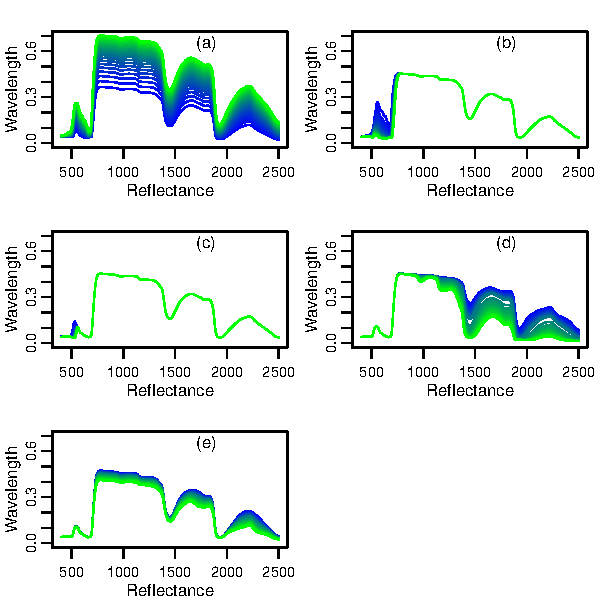
\includegraphics{figures/sensitivity}}
  \caption{
  Sensitivity of PROSPECT modeled reflectance to parameter values: (a) N, (b) 
  Cab, (c) Car, (d) Cw, and (e) Cm. Values increase from blue to green.
  }
  \label{fig:prospectsens}
\end{figure}

\subsection{Inversion procedure} \label{ss:m-inversion}

The complexity and non-linearity of the PROSPECT 5 model precludes an 
analytical solution for the parameters as a function of reflectance. Instead, 
we performed a statistical inversion, wherein the residual error between 
modeled and observed reflectance is modeled. This analysis was performed 
within a Bayesian framework, such that the result was a joint probability 
distribution of each PROSPECT 5 parameter and the residual error informed by 
prior expectations. The general mathematical statement of this posterior 
distribution is given as follows:

\begin{align}
  P(\theta, \sigma | \mathbf{X}) &\propto P(\mathbf{X} | \theta, \sigma) 
  P(\theta) P(\sigma) \\
  P(\mathbf{X} | \theta, \sigma) &= \mathit{Normal}(\mathrm{PROSPECT 5}(\theta) | \mathbf{X}, \sigma)
  \label{eq:bayes}
\end{align}

, where $\theta$ is the vector of PROSPECT 5 parameters, $\sigma$ is the 
residual standard deviation, $\mathrm{PROSPECT 5}(\theta)$ is the simulated
reflectance given $\theta$, and $\mathbf{X}$ is a vector of observed 
reflectance values. The residual error is assumed to be normally distributed 
with a mean of 0 and standard deviation $\sigma$. 

We set prior distributions on the PROSPECT 5 parameters to accommodate their
strict lower bounds (1 for N, 0 for Cab, Car, Cw, and Cm) while maintaining
approximately equal and low probability density over the entire range of
realistic values. We set the prior distribution for N to a lognormal
distribution shifted horizontally to have a minimum at 1 and parameterized
based on a review of literature featuring the PROSPECT model (e.g.
\cite{LeMaire2004,Ferreira2013,Croft2014}). We assigned the remaining
parameters log-normal priors based on summary statistics and histograms from
four spectral databases presented by Feret et al. (\cite{Feret2008}). The
residual variance $\sigma^2$ was assigned an uninformative inverse gamma
prior, which is conjugate with the normal and therefore allows for Gibbs
sampling.

We sampled the joint posterior distribution of the PROSPECT 5 parameters using
the Metropolis-Hastings (MH) algorithm with adaptive block sampling
(\cite{Haario2001}). Samples were drawn from a multivariate normal
distribution with means conditioned on the current accepted values and the
covariance matrix $\mathbf{J}$ re-computed every 100 samples as follows:

\begin{align}
    \mathbf{R} &= \frac{\mathbf{S} \times a}{t} \\
    \mathbf{J} &= \mathbf{R} \times \mathbf{C} \times \mathbf{R}
\end{align}

, where $\mathbf{R}$ is a diagonal matrix of factors for scaling the 
correlation matrix $\mathbf{C}$, $\mathbf{S}$ is a diagonal matrix of the 
sample standard deviations of parameters for the current 100-sample block, $a$ 
is the fraction of samples from the current block that have been accepted, and
$t$ is the target acceptance rate (set to 0.44, as per \cite{Haario2001}).  We
initialized inversions at random values drawn from the prior distributions,
but to improve convergence, these initial values were then optimized using the
Levenberg-Marquhardt (LM) algorithm prior to starting the Metropolis-Hastings
algorithm. Doing this worked for the majority of cases; however, for a small
subset of runs, the LM algorithm picked unrealistically large values (e.g. N >
20, Cab > 1000), causing the subsequent inversion to fail to converge on the
known correct values. When we skipped the initial LM optimization, the
inversion took longer to converge but never failed to converge (results not
shown). We assessed convergence and determined the burn-in period by visually
analyzing trace plots of the MH samples. We determined the thinning interval
by visually examining the autocorrelograms.  For each inversion, we calculated
the mean, standard deviation, median, and 95\% confidence intervals of the
sampled parameter values.  

The inversion algorithm described above is available as an open-source,
publicly-available R (\cite{Rcore}) package housed as a module within the
PEcAn ecoinformatics toolbox
(\url{github.com/PecanProject/PEcAn/modules/rtm}). Our package allows users to
simulate spectra using the PROSPECT and PROSAIL family of radiative transfer
models and apply our inversion algorithm to their own models and data. For
more information, see the package vignette.


\subsection{Validation} \label{ss:m-validation}

We performed two different tests to evaluate the accuracy of our inversion of
measured leaf spectra. First, we used the mean parameter estimates from each
leaf spectrum inversion to generate simulated reflectance and transmittance
spectra and compared these simulations to measured reflectance and
transmittance. The use of transmittance makes this approach robust, as the
inversions were performed on only reflectance data. For both reflectance and
transmittance, we plotted the mean and 90\% and 95\% confidence intervals on
the absolute error (simulated $-$ measured) at each wavelength. To facilitate
comparison with other RTM inversion studies (e.g. \cite{Feret2008,
DiVittorio2009}), we also computed the following statistics aggregated across
the visible (VIS, \SIrange{400}{800}{\nano\meter}) and near-infrared (NIR,
\SIrange{801}{2500}{\nano\meter}) regions of the spectrum: 

\begin{align}
  \mathrm{RMSE} &= \sqrt{\frac{\sum_n{\left(x_{\mathrm{sim}} - x_{\mathrm{obs}} \right)^2}}{n}} \\
  \mathrm{BIAS} &= \frac{\sum_n{\left(x_{\mathrm{sim}} - x_{\mathrm{obs}} \right)}}{n} \\
  \mathrm{SEPC} &= \sqrt{\frac{\sum_n{\left(x_{\mathrm{sim}} - x_{\mathrm{obs}} - \mathrm{BIAS}\right)^2}}{n}} \\
  \mathrm{CV} &= \frac{\mathrm{SEPC}}{x_{\mathrm{obs}}} \\
  \mathrm{RMSFE} &= \sqrt{\frac{\sum_n{\left(\frac{x_{\mathrm{sim}} - x_{\mathrm{obs}}}{x_{\mathrm{obs}}}\right)}}{n}}
\end{align}

, where $x_{\mathrm{sim}}$ is the simulated value (reflectance or
transmittance), $x_{\mathrm{obs}}$ is the observed value, and $n$ is the
number of spectra considered.

Second, we compared the mean inversion estimates for Cw and Cm to measured
values of EWT and LMA, respectively, for leaves where both inversion estimates
and measured values were available. For each, we plotted the measured value
against the inversion estimate and computed the same set of statistics as
above.

During exploratory analysis, we observed strong differences between the
results for broadleaved and needle-leaved species. Therefore, to better
contextualize our results, we performed both validation steps for the entire
data set and separately for broadleaved and needle-leaved species.

\subsection{Exploration of the sensor effect} \label{ss:m-sensor-effect}

To investigate the effect of spectral resolution on inversion accuracy and
precision, we simulated reflectance spectra using the PROSPECT 5 model,
transformed these spectra using the spectral response functions of 11 common
remote sensing platforms (Table \ref{tab:sensor-info}), and attempted to
retrieve the starting parameters from the transformed spectra. (We note that
this was done purely for illustration purposes; studies seeking to perform RTM
inversion on real remote sensing data should use a more complicated RTM that
accounts for canopy structure and possible sun-sensor geometry and atmosphere
rather than a simple leaf RTM as we do here.)  For input parameters, we used
the inversion results from measured spectra, thereby capturing a large range
of ecologically realistic values and preserving inherent covariances between
parameters. We then examined how two characteristics of the inversions varied
between sensors: Inaccuracy ($\alpha$) indicates how closely the mean parameter
estimate matched the true value, and uncertainty ($\pi$) indicates the
uncertainty in the inversion's parameter estimate.

\begin{align}
  \alpha &= \frac{\mu - p}{p} \\
  \pi &= \frac{\sigma}{\mu}
\end{align}

, where $\mu$ is the mean parameter estimate, $\sigma$ is the standard
deviation of the parameter estimate, and $p$ is the true parameter value. We
note that both statistics are normalized to facilitate inter-parameter
comparison. Both metrics were computed for each parameter for each inversion
and then averaged over the full range of results.

% Table of sensor information
% Fri Jul 31 20:36:03 2015
\begin{table}[ht]
  \centerline{
\begin{tabular}{cccccc}
  \hline
  Sensor   &   Bands\tablefootnote{Excluding values outside \SIrange{400}{2500}{\nano\meter} range and panchromatic bands} &   Spectral range (\si{\nano\meter})   &   Bandwidth (\si{\nano\meter})   &   Spatial resolution (\si{\meter})   &   Revisit time (days) \\
  \hline
  AVIRIS NG        &   416   &   \numrange{380}{2510}   &   5                     &   \numrange{0.3}{4.0}   &   On-demand only \\
AVIRIS Classic     &   216   &   \numrange{400}{2500}   &   \SI{10}               &   20                    &   On-demand only \\
CHRIS-Proba        &   62    &   \numrange{410}{1050}   &   \numrange{1.5}{12}    &   36                    &   \numrange{7}{8} \\
Hyperion           &   225   &   \numrange{350}{2500}   &   10                    &   30                    &   16 \\
  Landsat 5 TM     &   6     &   \numrange{450}{2350}   &   \numrange{60}{270}    &   30                    &   16 \\
  Landsat 7 ETM+   &   6     &   \numrange{440}{2350}   &   \numrange{60}{280}    &   30                    &   16 \\
  Landsat 8 OLI    &   8     &   \numrange{435}{2295}   &   \numrange{20}{185}    &   30                    &   16 \\
  MODIS (Terra)    &   7     &   \numrange{459}{2155}   &   \numrange{20}{50}     &   \numrange{250}{500}   &   \numrange{1}{2} \\
  VIIRS            &   10    &   \numrange{402}{2275}   &   \numrange{15}{60}     &   750                   &   \numrange{1}{2} \\
  AVHRR            &   3     &   \numrange{580}{1640}   &   \numrange{100}{275}   &   1090                  &   1 \\
   \hline
\end{tabular}
}
\caption{Spectral, spatial, and temporal characteristics of sensors considered in this study.} 
\label{tab:sensor-info}
\end{table}

The data and R source code for performing all analyses in this study is
publicly available at
\url{github.com/ashiklom/prospect_bayes/sensor-manuscript}. We encourage
 interested readers to replicate our analyses and build on them with their own
data and models.
\section{Results and discussion} \label{s:results}

\subsection{Validation}

\subsubsection{Reflectance and transmittance} \label{sss:refltrans}

\begin{figure}[h] \centering
  \centerline{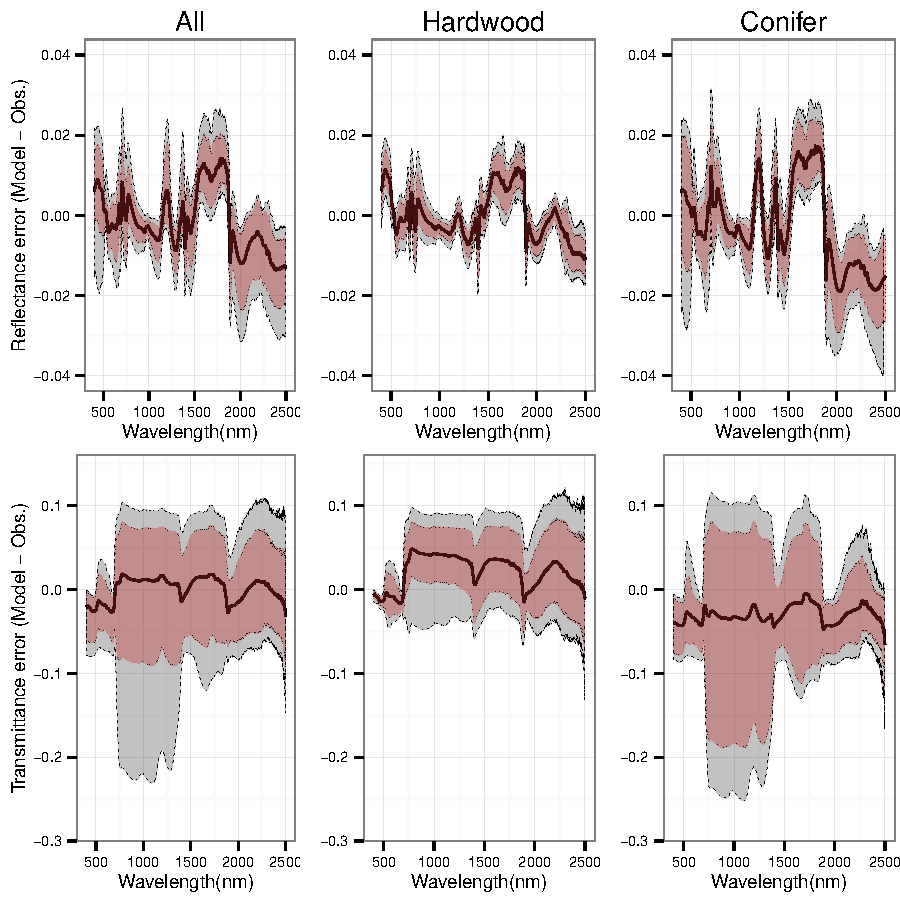
\includegraphics{figures/refltrans-validation}}
  \caption{
    Errors in reflectance (top) and transmittance (bottom) spectra simulated
    using PROSPECT 4 parameters from the inversion output for all leaves(left)
    and only hardwood (middle) and conifer (right) species. For a given
    wavelength, the solid black line is the mean error, the red region bounded
    by the dotted line is the 90\% confidence interval on the error, and the
    grey region bounded by the dashed line is the 95\% confidence interval.
  }
  \label{fig:refltrans}
\end{figure}

Figure \ref{fig:refltrans} shows the results of the validation based on
comparison of observed and simulated reflectance and transmittance spectra.
At the scale of the entire data set, statistically significant reflectance
errors occurred in the near and short wave infrared region, with overestimates
in the \SIrange{1500}{1900}{\nano\meter} range and underestimates at around
\SIlist{1100;2000;2400}{\nano\meter}.  For broadleaved species, significant
differences in reflectance were overestimates around \SI{450}{\nano\meter} and
in the \SIrange{1500}{1900}, while needle-leaved reflectance was overestimated
around \SI{1700}{\nano\meter}.  Other prominent reflectance errors lined up
with spectral ``edges''--i.e.  large changes in reflectance over a small
number of wavelengths, such as the chlorophyll absorption ``green edge'' or
the leaf structural scattering ``red edge''--but none of these errors were
significantly different from zero.

Errors in transmittance were, on average, greater than those for reflectance,
with mean transmittance mostly overestimated for broadleaved species and
underestimated for needle-leaved species. However, the variability in these
errors was also very large, meaning that statistically significant
($p < 0.05$) errors occurred in only a few very specific regions of the spectrum:
Around \SI{450}{\nano\meter}, corresponding to chlorophyll a absorption;
around \SI{700}{\nano\meter}, corresponding to the vegetation ``red edge'';
and, for needle-leaved species, around \SI{1900}{\nano\meter}, corresponding
to a water absorption feature.

Our study is not the first to report issues with modeling reflectance and
transmittance in the \SIrange{400}{450}{\nano\meter} range.  Feret et al.
\cite{Feret2008} observed a consistently negative transmittance bias and
occasionally a positive or negative reflectance bias.  Similarly, Croft et al.
\cite{Croft2013} report systematic underestimates of reflectance in this
region. Most likely, these biases are the result of the failure of the
PROSPECT model to distinguish between chlorophyll a and b, which
have overlapping but distinctly different absorption signatures and whose
ratios have been shown to be affected by environmental conditions
(\cite{Blackburn2007, DiVittorio2009b, DiVittorio2009a}).  Fortunately, it has
been shown that not only can chlorophyll a and b be distinguished using
imaging spectroscopy (\cite{DiVittorio2009a}), but that these differences can
be incorporated into a radiative transfer model to improve its performance
(\cite{DiVittorio2009}).  As such, we argue that future development of
PROSPECT and other radiative transfer models should include this distinction.

The large variability in transmittance errors is most likely driven by the
fact that our inversion procedure targeted only reflectance. If we had used
both reflectance and transmittance data, we would expect to see the
variability distributed more evenly. That being said, the inherent challenges
of measuring transmittance--especially related to the expense and insufficient
quality of integrating spheres--likely contribute to substantially higher
uncertainties in the measured transmittance. This is supported by the absence
of significant systematic bias between measured and modeled transmittance
(except in the regions discussed above).  Furthermore, although the confidence
intervals in Figure \ref{fig:refltrans} appear very large, when averaged over
the visible (\SIrange{400}{800}{\nano\meter}) and infrared
{\SIrange{801}{2500}{\nano\meter}) regions, the resulting statistics are at
least comparable to--and often better than--those reported in other field
spectra inversion studies (Table \ref{tab:refltrans}).  Although our overall
transmittance RMSE values were higher than that reported by \cite{Feret2008},
these errors are inflated by the inclusion of needle-leaved species, whose
reflectance is harder to measure reliably and which do not satisfy the
assumptions of the PROSPECT model.  When looking only at hardwoods, our
statistics for transmittance were fully comparable to \cite{Feret2008},
despite the fact that we did not use any transmittance information to perform
the inversion.  When compared with transmittance error statistics reported for
conifers by \cite{DiVittorio2009}, our values are of very similar magnitude,
even despite the fact that \cite{DiVittorio2009} used the more
needleleaf-friendly LIBERTY model.  Moreover, our reflectance error statistics
are consistently comparable to or lower than those reported in comparable
studies (\cite{Feret2008, DiVittorio2009}.

% latex table generated in R 3.2.1 by xtable 1.7-4 package
% Fri Aug 14 16:30:07 2015
\begin{table}[ht]
\centerline{
\begin{tabular}{rrrrrrr}
  \hline
 & VIS-RMSE & VIS-BIAS & VIS-SEPC & IR-RMSE & IR-BIAS & IR-SEPC \\ 
  \hline
All-R & 0.0077 & 0.0019 & 0.0064 & 0.0095 & -0.0021 & 0.0056 \\ 
  Hardwood-R & 0.0062 & 0.0023 & 0.0040 & 0.0062 & -0.0009 & 0.0030 \\ 
  Conifer-R & 0.0092 & 0.0014 & 0.0079 & 0.0123 & -0.0036 & 0.0057 \\ 
  All-T & 0.0403 & -0.0133 & 0.0335 & 0.0551 & 0.0041 & 0.0536 \\ 
  Hardwood-T & 0.0248 & 0.0012 & 0.0167 & 0.0450 & 0.0266 & 0.0336 \\ 
  Conifer-T & 0.0553 & -0.0345 & 0.0389 & 0.0660 & -0.0291 & 0.0565 \\ 
   \hline
\end{tabular}
}
\caption{ Modeled reflectance (R) and transmittance (T) error statistics. } 
\label{tab:refltrans}
\end{table} 

\subsubsection{EWT and LMA}

Figures \ref{fig:water} and \ref{fig:lma} compare inversion parameter
estimates and direct measurements for equivalent water thickness (EWT;
PROSPECT parameter Cw) and leaf mass per unit area (LMA; PROSPECT parameter
Cm), respectively. Table \ref{tab:water-lma} shows the relevant summary
statistics for both. 

Echoing the results of the spectral validation (section \ref{sss:refltrans}),
parameter estimates were much more accurate for broadleaved than needleleaved
species, and the relevant statistics for broadleaved species agree with those
reported by others (\cite{Feret2008, Li2011a}.  Interestingly, the strongest
overestimates for both EWT and LMA occur in early successional needleleaf
species, which for this data set consisted entirely of pine species
(\textit{Pinus} family). One explanation for this is the unique methodological
challenge of measuring pine needle reflectance using a leaf-clip setup, as
multiple needles are required to completely cover the spectroradiometer lens
and the rounded shape of pine needles (compared to the flatter shape other
conifer families) may artificially dampen the measured reflectance, thereby
leading to parameter overestimation. Alternatively, the overestimation may be
the result of saturation in the response of PROSPECT to its parameters; i.e.
as parameters get larger, it becomes harder to distinguish between them (See
Figure \ref{fig:prospectsens}).  

The persistent negative bias we found in spectral estimates of LMA for
broadleaved species has been reported elsewhere but inconsistently so, with
some studies showing negative bias across all their data (\cite{Li2011a,
Cheng2014}) and others reporting a bias whose magnitude and direction is
data-dependent (\cite{Feret2008}). This may partially be explainable by the
simplicity of PROSPECT's treatment of leaf structural components;
specifically, protein, cellulose, hemicellulose, sugar, starch, and lignin are
aggregated into a single parameter (Cm) (\cite{Fourty1996}) based on the sum
of their absorption features.  As with chlorophyll, this fails to take into
account variability in the relative abundance of the different components,
which varies substantially in response to environmental conditions
(\cite{Poorter2009}).  Furthermore, measurements of LMA are likely to
inadvertently include additional components such as chlorophyll, carotenoids,
lipids, organic acids, phenolics, and vascular tissue (\cite{Poorter2009}),
which would positively bias the measurement compared to the spectral estimate.
Similarly, as a spectral parameter, Cm is driven by the area over which
absorption can take place, which is affected by the geometry of absorbing
structural materials in the leaf and may therefore be slightly larger than the
actual measured leaf area; this would also negatively bias the inversion
estimate.  Finally, it is possible that the inversion is confused by the
significant overlap in the spectral effects of scattering by multiple layers
(N parameter) and absorption by leaf structural components (Cm parameter)
(Figure \ref{fig:prospectsens}), which results in strong positive covariance
in the sampling of these two parameters (Figure \ref{fig:pairs4}).  We are
aware of only one other study that attempted to estimate all five PROSPECT
parameters simultaneously: Li and Wang (\cite{Li2011a}) presented a novel
algorithm for PROSPECT inversion that assigns a separate merit function to
each parameter and demonstrated its improved performance over traditional
approaches.  However, although their new algorithm reduced error and bias in
the LMA estimates, a negative bias comparable to the one we report still
remained across all of their data sets. 

\begin{figure}[h]
  \centering
  \centerline{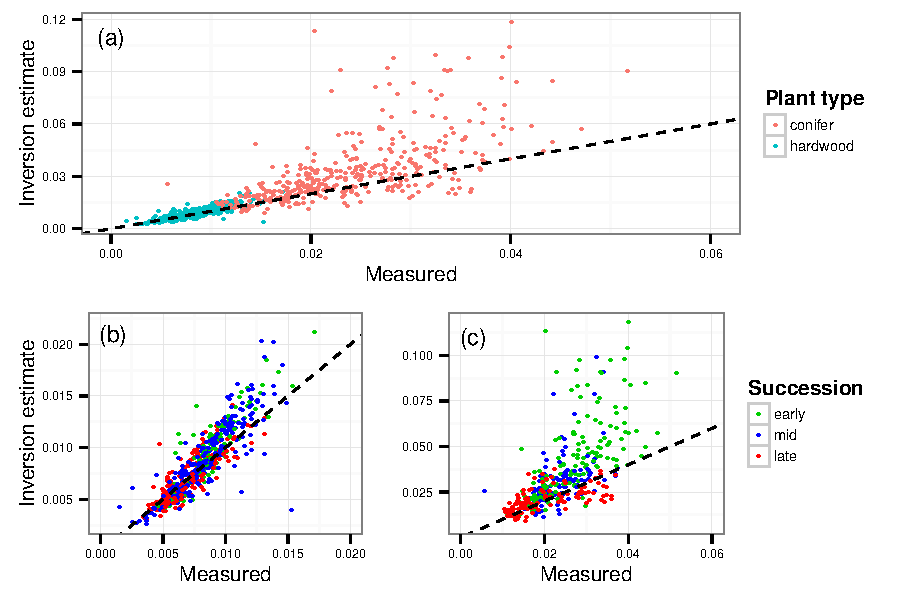
\includegraphics{figures/water}}
  \caption{
    Modeled and observed equivalent water thickness for both conifers and 
    hardwoods (a), just hardwoods (b), and just conifers (c). Point colors 
    indicate plant type (a) or successional stage (b,c). The dashed line 
    represents a 1:1 fit.
    }
  \label{fig:water}
\end{figure}

\begin{figure}[h]
  \centering
  \centerline{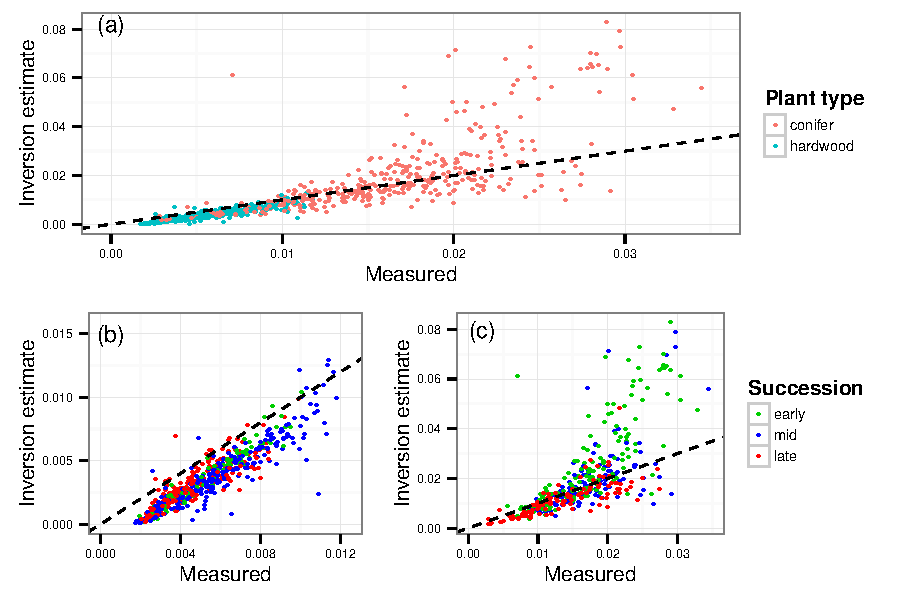
\includegraphics{figures/lma}}
  \caption{
    Modeled and observed leaf mass per unit area (g cm-2) for both conifers 
    and hardwoods (a), just hardwoods (b), and just conifers (c). Point colors 
    indicate plant type (a) or successional stage (b,c). The dashed line 
    represents a 1:1 fit.
    }
  \label{fig:lma}
\end{figure}

% latex table generated in R 3.2.1 by xtable 1.7-4 package
% Fri Aug 14 16:30:08 2015
\begin{table}[ht]
\centerline{
\begin{tabular}{llrrrrr}
  \hline
Parameter & Plant type & RMSE & BIAS & SEPC & CV & RMSPE \\ 
  \hline
EWT & conifer & 0.0191 & 0.0091 & 0.0168 & 0.5324 & 0.6930 \\ 
  EWT & hardwood & 0.0017 & 0.0005 & 0.0016 & 0.1880 & 0.2162 \\ 
  LMA & conifer & 0.0125 & 0.0036 & 0.0119 & 0.6330 & 0.6712 \\ 
  LMA & hardwood & 0.0020 & -0.0018 & 0.0009 & 0.2450 & 0.4375 \\ 
   \hline
\end{tabular}
}
\caption{ Error statistics for equivalent water thickness (EWT) and leaf mass per unit area (LMA) model estimates compared to inversion. } 
\label{tab:water-lma}
\end{table}

\subsection{Effect of sensor}

Table \ref{tab:sensor} summarizes the results of the sensor simulation
experiment by showing the mean inaccuracy and uncertainty for each sensor.

% latex table generated in R 3.2.1 by xtable 1.7-4 package
% Fri Aug 14 16:30:08 2015
\begin{table}[ht]
\centerline{
\begin{tabular}{lrrrrrrrrrr}
  \hline
Sensor & $\pi(\mathrm{N})$ & $\pi(\mathrm{Cab})$ & $\pi(\mathrm{Car})$ & $\pi(\mathrm{Cw})$ & $\pi(\mathrm{Cm})$ & $\alpha(\mathrm{N})$ & $\alpha(\mathrm{Cab})$ & $\alpha(\mathrm{Car})$ & $\alpha(\mathrm{Cw})$ & $\alpha(\mathrm{Cm})$ \\ 
  \hline
ASD Field Spec & 0.0008 & 0.0015 & 0.0065 & 0.0009 & 0.0038 & -0.0001 & -0.0001 & -0.0002 & -0.0001 & -0.0000 \\ 
  AVIRIS NG & 0.0036 & 0.0073 & 0.0339 & 0.0041 & 0.0191 & -0.0021 & -0.0019 & -0.0031 & -0.0019 & -0.0001 \\ 
  AVIRIS Classic & 0.0064 & 0.0138 & 0.0681 & 0.0074 & 0.0358 & -0.0049 & -0.0044 & -0.0088 & -0.0045 & 0.0015 \\ 
  Hyperion & 0.0062 & 0.0138 & 0.0702 & 0.0071 & 0.0356 & -0.0053 & -0.0047 & -0.0030 & -0.0050 & 0.0008 \\ 
  CHRIS-Proba & 0.0000 & 0.0000 & 0.0000 & 0.0000 & 0.0002 & 0.0000 & 0.0000 & 0.0000 & 0.0000 & 0.0000 \\ 
  Landsat 5 & 0.0287 & 0.0560 & 0.2795 & 0.0488 & 0.2011 & -0.0336 & -0.0353 & -0.0278 & -0.0116 & 0.3628 \\ 
  Landsat 7 & 0.0288 & 0.0649 & 0.3196 & 0.0470 & 0.2005 & -0.0344 & -0.0250 & -0.0833 & -0.0152 & 0.3312 \\ 
  Landsat 8 & 0.0242 & 0.0513 & 0.3110 & 0.0477 & 0.1204 & -0.0242 & -0.0222 & -0.0510 & -0.0125 & 0.1736 \\ 
  MODIS & 0.0310 & 0.0466 & 0.5450 & 0.0505 & 0.2453 & -0.0392 & -0.0437 & 0.0896 & -0.0445 & 0.3070 \\ 
  VIIRS & 0.0135 & 0.0408 & 0.4150 & 0.0187 & 0.0726 & -0.0153 & -0.0082 & -0.0938 & -0.0105 & 0.0793 \\ 
  AVHRR & 0.0702 & 0.3045 & 0.7243 & 0.2141 & 0.4815 & -0.0191 & -0.0884 & -0.3566 & -0.0429 & 1.8278 \\ 
   \hline
\end{tabular}
}
\caption{ Mean inaccuracy ($\alpha$) and uncertainty ($\pi$) by sensor. } 
\label{tab:sensor}
\end{table}

\subsubsection{Parameter error}

Figure \ref{fig:sensor-error} compares known parameter values and inversion
estimates for simulated spectra filtered through the spectral response
functions of various sensors. The spectral resolution of the four
hyperspectral sensors (AVIRIS NG, AVIRIS Classic, Hyperion, CHRIS-Proba) was
sufficient to accurately estimate all parameters, although gradually declining
spectral resolution resulted in increasingly large underestimates at the upper
end of the range.  The ability of CHRIS-Proba to retrieve all parameters with
high accuracy and low uncertainty is particularly noteworthy because although
it has a relatively high spectral resolution, it also has a much shorter
spectral range than any of the other sensors and avoids the pitfalls of
measuring in the generally noisier SWIR regions of the spectrum.  At coarser
spectral resolution, inversion accuracy becomes much more parameter-dependent,
corresponding to the extent to which parameter spectral features line up with
sensor bands. For instance, all of the sensors at this range do a reasonable
job of estimating water content, but the greater number of Landsat bands in
the visible range improves their ability to estimate chlorophyll and
carotenoids compared to MODIS, VIIRS, and AVHRR. This analysis is also able to
shed light on differences between sensors with similar missions (e.g.  Landsat
5 vs 7 vs 8; MODIS vs VIIRS). For example, greater number of usable land bands
on VIIRS compared to MODIS drives its superiority for estimating all
parameters except carotenoids, which are highly sensitive to the width and
location of bands in the visible range. Similarly, none of the Landsat sensors
appear unequivocally superior to any of the others; Landsat 8 performs best
for estimating N, Cab, and Cm, while the wider visible bands on Landsat 5
afford it the highest accuracy and lowest uncertainty for Car (That being
said, we did not consider the much improved radiometric resolution of Landsat
8, which should afford it a huge advantage over older Landsat sensors in real
situations).  Lastly, it is worth noting that despite having only three broad
bands originally intended only for meteorology and not studying the land
surface (let along inverse radiative transfer modeling!), AVHRR is still able
to provide some information about leaf chlorophyll and water content.

A critical caveat to these results is that they are highly theoretical. All
they are showing is the effect of the sensors' spectral resolution on the
ability to estimate leaf-level radiative transfer parameters. To use actual
measurements from these sensors in an inverse radiative transfer modeling
capacity, other factors such as radiometric resolution, spatial resolution,
atmospheric conditions, and sun-sensor geometry must be taken into account as
they may influence the information content of the data more than spectral
resolution alone.

\begin{figure}[h] \centering
  \centerline{ 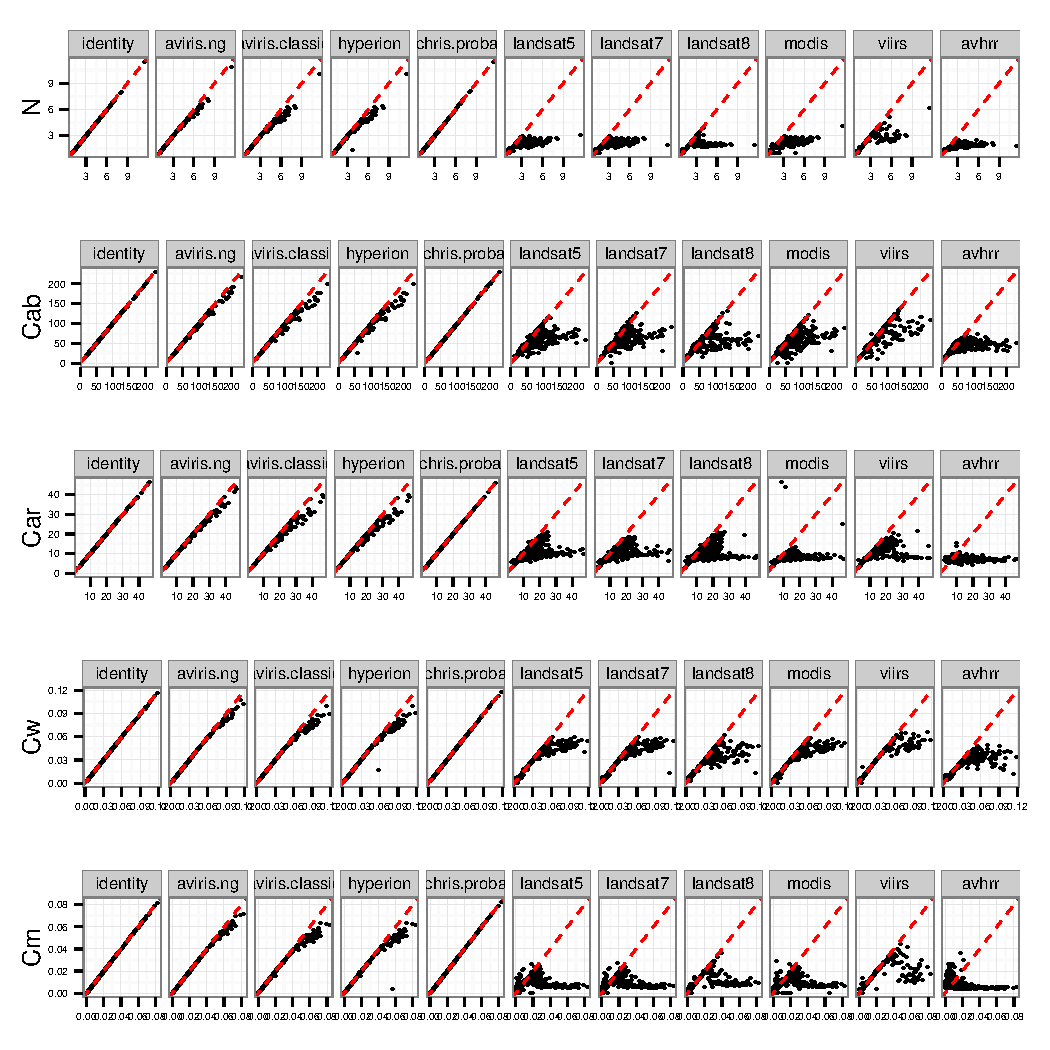
\includegraphics{figures/sensor-error}} 
  \caption{
    Parameter inversion estimates as a function of true values for the 
    spectral response functions of different sensors. The dashed red line is a 
    1:1 fit.
  }
  \label{fig:sensor-error}
\end{figure}

\subsubsection{Parameter uncertainty and covariance}

Figure \ref{fig:pairs-4} shows an example of processed output of inversions
based on full field spectra and the spectral response functions of AVIRIS NG,
Landsat 8, and MODIS. All four plots are simulated from a single set of
parameters, so differences in results are caused only by variations in the
quality of the spectra. Out of these four sensors, the smallest overall
uncertainties are in the full spectra, and the second-smallest are in the
AVIRIS NG spectra, while the uncertainties for Landsat 8 and MODIS are
comparable overall but strongly parameter dependent.  More importantly, the
shapes of parameter covariances are distinctly different between these
sensors, reflecting differences in the inversion's ability to distinguish
between parameters based on the available information.  Across all four of
these sensors, we observe negative covariance between Cw and Cm, which makes
sense given the spectral overlap between these parameter pairs in the SWIR
(Figure \ref{fig:prospectsens}). The full spectra, AVIRIS NG, and MODIS share
a strong positive covariance between N and Cm, but this covariance is largely
absent in Landsat 8, presumably because at least one Landsat band is only
affected by N and not Cm. On the other hand, Landsat has a strong negative
covariance between Cab and Car because the precise location of its visible
bands limits its ability to distinguish between these two spectrally-proximate
parameters. Similarly, MODIS has a strong negative covariance between N and
Cw, which, considered together with the strong N-Cm and Cw-Cm covariances is a
symptom of its weakness at measuring in the SWIR.

\begin{figure}[h] \centering
  \centerline{ 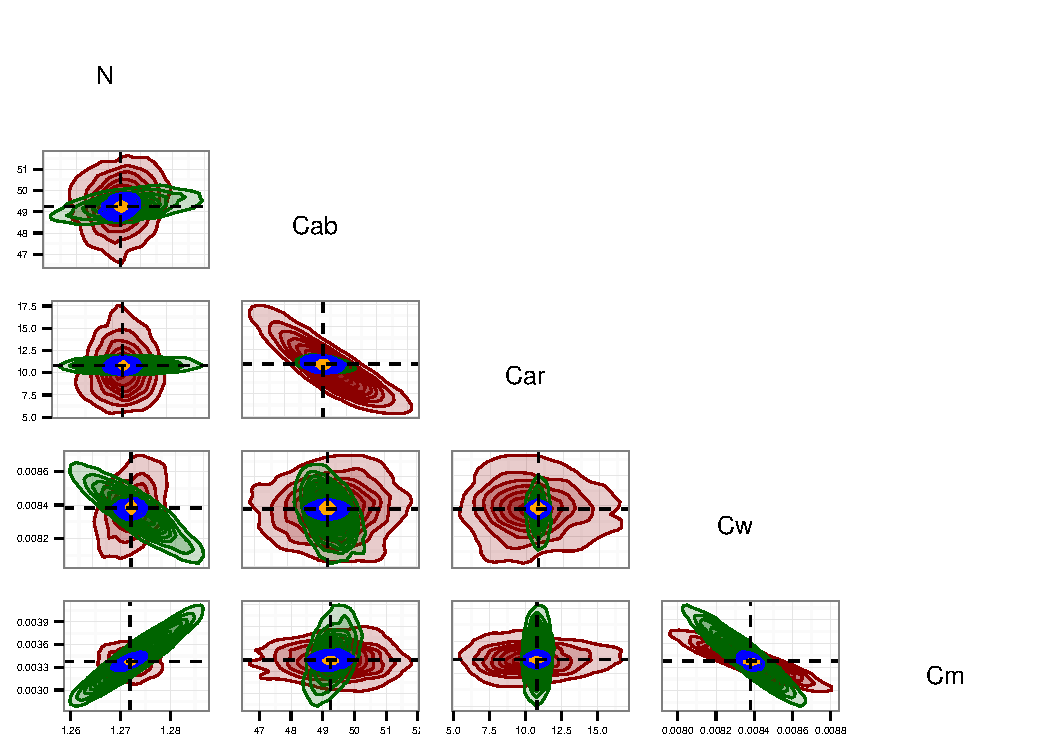
\includegraphics{figures/pairs-4}} 
  \caption{
    Joint probability distribution for parameter inversion estimates of 
    simulated spectra using the full spectra (orange) and the spectral
    response functions of AVIRIS NG (blue), MODIS (green), and Landsat 8
    (red). Dotted lines indicate true parameter values.
  }
  \label{fig:pairs-4}
\end{figure}
\include{discussion}
\section{Conclusions} \label{s:conclusions} 

This paper demonstrates a novel approach to performing radiative transfer
model inversion that explicitly takes into account uncertainty and covariance
in parameter estimates. Our validation shows that the accuracy of our method
is comparable to that of other studies when using field spectra. Our idealized
sensor simulation exercise clearly demonstrated how the spectral configuration
of different sensors affects their ability to inform different RTM parameters.
Although our finding that RTM inversion accuracy and precision increase with
spectral resolution is not surprising, we highlght the fact that by combining
the spectral information content of just two multispectral sensors like
Landsat and MODIS, we dramatically improve our inversion estimates. We hope
our work will be integrated into existing approaches to multi-temporal,
multi-sensor retrieval of vegetation parameters to enhance our capability to
observe vegetation remotely and enhance our understanding of ecosystem
processes.

%% References
\bibliographystyle{plain}
\bibliography{sensor-manuscript.bib}

\end{document}